\documentclass[openany,fontset=none]{intromech}

%\usepackage{showkeys}

\begin{document}
%
\newboolean{makeall}
\setboolean{makeall}{true}
\newcounter{makechapter}
\setcounter{makechapter}{2}

\ifthenelse{\boolean{makeall}}{
% 封面
\includepdf{body/F00-frontpage.pdf}

% 标题页
\includepdf{body/F01-titlepage.pdf}

% 出版信息页
\input{body/F02-publishinfo}

% 内容提要
\input{body/F03-abstract}

% 序言
\input{body/F04-foreword}

% 目录
\clearpage
\setcounter{page}{1}
\tableofcontents
}{}

% 正文
\clearpage
\pagestyle{heading}
\setcounter{page}{1}
% 公式与上下文本距离调整
\setlength\abovedisplayskip{1pt plus 3pt minus 1pt}
\setlength\belowdisplayskip{1pt plus 3pt minus 1pt}

% 绪论
\ifthenelse{\boolean{makeall} \OR \(\value{makechapter}=0\)}{
\input{body/M00.00-Introduction.tex}
}{}

% 第一章
\ifthenelse{\boolean{makeall} \OR \(\value{makechapter}=1\)}{
\chapter{时间,空间和运动学}\label{chp:01}

\input{body/M01.01-Time, Space and Kinematics.tex}
\input{body/M01.02-Time, Space and Kinematics.tex}
\input{body/M01.03-Time, Space and Kinematics.tex}
\input{body/M01.04-Time, Space and Kinematics.tex}
\input{body/M01.05-Time, Space and Kinematics.tex}
\input{body/M01.06-Time, Space and Kinematics.tex}
\input{body/M01.07-Time, Space and Kinematics.tex}
\section{加速度}\label{sec:01.08}

为了描写速度的变化,我们再引入一个物理量,即所谓加速
度。对于直线运动,若当$t$时刻,质点速度为$v(t)$,$当t+\Delta t$时
刻,为$v(t+\Delta t)$,则我们定义从$t$到$t+\Delta t$间隔中质点的平均加
速度为
\begin{equation}\label{equ:01.08.01}
    \langle a\rangle_{t\rightarrow t+\Delta t} = \frac{v(t+\Delta t)-v(t)}{\Delta t}
\end{equation}
它的定义是质点在单位时间中速度的平均变化,单位是$\text{米/秒}^2$。

利用式\eqref{equ:01.06.02},可以计算自由落体在$t$到$t+\Delta t$间隔中的平
均加速度:
\begin{equation*}
    \begin{aligned}
        \langle a\rangle_{t\rightarrow t+\Delta t} & = \frac{9.8(t+\Delta t)-9.8t}{\Delta t} \\
                                                   & = 9.8\text{米/秒}^2
    \end{aligned}
\end{equation*}
这个结果中不含$t$和$\Delta t$,也就是说,对任何一段时间间隔,自由落
体的平均加速度都是一样的。这种加速度不随时间变化的运动,
称为匀加速运动。自由落体运动是一个典型的匀加速运动。无论
用何种材料作成的物体,它的自由落体加速度总等于9.8~$\text{米/秒}^2$。
称此加速度为重力加速度,用$g$表示。

精确测量表明,在地球各处,重力加速度$g$并不都一样,一
\begin{tablex}[!b]{2em}
    \caption{地球上不同地点的$g$值}
    \label{tab:01.06}
    \centering
        \begin{tabular}{l|l|S}
            \toprule
            地~~点             & 纬~~~度      & $g$(米/秒) \\
            \midrule
            北~~极             & 北纬\ang{90} & 9.83245      \\
            戈拉雅克(格陵兰)   & 北纬\ang{70} & 9.8253       \\
            雷克雅未克(冰岛)   & 北纬\ang{64} & 9.8227       \\
            列宁格勒           & 北纬\ang{60} & 9.8193       \\
            巴~~黎             & 北纬\ang{49} & 9.8094       \\
            北~~京             & 北纬\ang{40} & 9.8012       \\
            汉~~口             & 北纬\ang{30} & 9.7936       \\
            广~~州             & 北纬\ang{23} & 9.7883       \\
            蒙罗维亚(利比里亚) & 北纬\ang{6}  & 9.7816       \\
            雅加达             & 南纬\ang{6}  & 9.7813       \\
            墨尔本             & 南纬\ang{38} & 9.7999       \\
            \bottomrule
        \end{tabular}
\end{tablex}
\clearpage
\noindent 般说来,在低纬度处$g$值较小;在高纬度处,$g$值较大(表\ref{tab:01.06})。

类似于平均速度不足以细致地描写非匀速运动一样,平均加
速度也不足以细致地描写非匀加速运动。对于非匀加速运动,必
须引入瞬时加速度来描述它的速度变化。加速度也是一个描述运
动的瞬时性质的物理量。瞬时加速度定义为:
\begin{equation*}
    \begin{aligned}
        a(t) & =\lim _{\Delta t \rightarrow 0} \frac{v(t+\Delta t)-v(t)}{\Delta t} \\
             & =\frac{dv(t)}{dt}=\frac{d^2 x(t)}{d t^2}
    \end{aligned}
\end{equation*}
它的意义是质点在时刻t的无限小时间间隔中的平均加速度。以
后我们谈到加速度,一般都是指瞬时加速度。

对于一般的曲线运动,可以给出相应的平均加速度及瞬时加
速度为:
\begin{equation}\label{01.08.02}
    \langle \vq{a} \rangle_{t \rightarrow t+\Delta t} = \frac{\vq{v}(t+\Delta t)-\vq{v}(t)}{\Delta t}
\end{equation}
\begin{equation}\label{01.08.03}
    \begin{aligned}
        \vq{a}(t) & =\lim _{\Delta t \rightarrow 0} \frac{\vq{v}(t+\Delta t)-\vq{v}(t)}{\Delta t} \\
                  & =\lim_{\Delta t \rightarrow 0}\frac{\Delta \vq{v}}{\Delta t}                  \\
                  & =\frac{d\vq{v}(t)}{dt}=\frac{d^2 \vq{r}(t)}{d t^2}
    \end{aligned}
\end{equation}
在曲线运动情况下,速度方向是变化的。$v(t)$,$v(t+\Delta t)$及$\Delta v$,
一般如图l-14所示。由于$a$平行于$\Delta v$,所以平均加速度的方向一
般与速度方向并不相同。瞬时加速度也类似。当加速度方向平行
于速度时,表示速度方向没有变化,但速率增加。当二者反平行
时,表示速度方向不变,而速率减少。当加速度既不平行也不反
平行于速度时,表示速度方向也在变化。

利用式\eqref{equ:01.07.03},加速度矢量的分量可以表示为:
\begin{equation}\label{equ:01.08.04}
    \vq{a}=\frac{d^2x(t)}{dt^2}\vq{i}+\frac{d^2y(t)}{dt^2}\vq{j}+\frac{d^2z(t)}{dt^2}\vq{k}
\end{equation}
加速度的三个坐标分量为:
\begin{equation}\label{equ:01.08.05}
    a_x=\frac{d^2x(t)}{dt^2},~ a_y=\frac{d^2y(t)}{dt^2},~
    a_z=\frac{d^2z(t)}{dt^2}
\end{equation}
$\vq{r}$,$\vq{v}$,$\vq{a}$是描写运动的物理量。我们希望用数目比较少的物
理量来描写运动。什么州比较步?意思是这些物理量之间应是相
互独立的。所谓相互独立。是说其中任一个量不能由其他的量加
以确定。用$\vq{r}$,$\vq{v}$及$\vq{a}$三个量来描写运动是必要的,因为它们是相互
独立的。例如,在某一时刻,知道了质点的位置$\vq{r}$,并不能知道
它的速度$\vq{v}$,知道了$\vq{v}$,也并不能知道$\vq{a}$,反之亦然。人们认识到
这一点,也并不容易。在伽利略之前,并没有加速度概念。当时,
没有人认识到加速度与速度是相互独立的,所以没有认识到需要
用加速度来描写运动。

我们已讨论了位置矢量、速度和加建度。从运动学本身来考
虑,没有足够的理由说明,为什么我们应当到此为止,而不去讨
论加加速度、加加加速度……。当然,我们可以定义并计算加加
速度,即加速度的变化率,但一般说这并不代表任何具有基本物
理价值的东西。其中的原因在动力学,学过动力学后,我们将看
到,对力学的讨论几乎全部是基于位置矢量,速度和加速度这三
个量。

下面我们介绍运动的独立性这一重要概念。由式\eqref{equ:01.05.02}、
\eqref{equ:01.07.03}、\eqref{equ:01.08.05}可以看到,描写一个复杂的曲线运动时,$X$方
向的坐标、速度、加速度与其他方向的坐标,速度、加速度无关。
$Y$方向和$Z$方向也有这种性质,即三个方向相互无关,这种性质被
称为运动的独立性。因此,一个复杂的曲线运动,可看成在$X$,$Y$,
$Z$三个方向上的直线运动,这三个运动同时进行,我们可以对每
一个运动进行单独的分析,好象另外两个自由度上的运动是根本
不存在一样,这样就使问题变得简单。

\example{1} 已知一个质点作直线运动。观察到它的位置与时间
的变化如表\ref{tab:01.07}所示。用这些数据求出各时间间隔的平均速度$v$及
平均加速度$a$,并写出运动方程式。
\begin{tablex}[!h]{0.6em}
    \caption{}
    \label{tab:01.07}
    \centering
    \begin{tabular}{l|c|c|c|c|c|c|c|c|c}
        \toprule
        时~~~~间(秒) & 0 & 1 & 2 & 3 & 4 & 5 & 6 & 7 & 8 \\
        \midrule
        \makecell{与参考点的距离                           \\(米)}  &  3  &  4  &  9  &  18  &  31  &  48  &  69  &  94 & 123 \\
        \bottomrule
    \end{tabular}
\end{tablex}

\solution 因为时间间隔都是1秒,即$\Delta t=1$秒。所以从数值上有
\begin{align*}
    v & =\frac{\Delta s}{\Delta t}=\Delta s                         \\
    a & =\frac{(v_2-v_1)}{\Delta}=v_2-v_1=(\Delta s_2)-(\Delta s_1)
\end{align*}
将结果列于表\ref{tab:01.08}中。
\begin{tablex}[!h]{0.2mm}
        \caption{}
        \label{tab:01.08}
        \centering \zihao{-5}
        \begin{tabular}{l|c|c|c|c|c|c|c|c|c|c|c|c|c|c|c|c|c}
            \toprule
            时~~~~间(秒)                              & 0 &   & 1 &   & 2 &   & 3  &    & 4  &    & 5  &    & 6  &    & 7  &    & 8   \\
            \midrule
            与参考点的距离(米)                        & 3 &   & 4 &   & 9 &   & 18 &    & 31 &    & 48 &    & 69 &    & 94 &    & 123 \\
            各秒内的位置变化($\Delta s$)(米)          &   & 1 &   & 5 &   & 9 &    & 13 &    & 17 &    & 21 &    & 25 &    & 29 &     \\
            各秒内的平均速度($v$)(米/秒)              &   & 1 &   & 5 &   & 9 &    & 13 &    & 17 &    & 21 &    & 25 &    & 29 &     \\
            各秒内的平均加速度($a$)($\text{米/秒}^2$) &   &   & 4 &   & 4 &   & 4  &    & 4  &    & 4  &    & 4  &    & 4  &    &     \\
            \bottomrule
        \end{tabular}
\end{tablex}

\noindent 既然平均加速度$a$是一个常数,所以这个直线运动是匀加速
直线运动,加速度是$a=4$米/秒$^2$.对于匀加速直线运动,一般的
运动方程是:
\begin{equation*}
    s=s_0+v_{0}t+\frac{1}{2}at^2
\end{equation*}
用已知数据代入,便可求出$s_0$,$v_0$,$a$。

当$t=0$时,$s=s_0=3$,所以$s_0=3$;

当$t=1$时,$4=3+v_0+\dfrac 1 2 a$,即$v_0+\dfrac 1 2 a=1$;

当$t=2$时,$9=3+2v_0+2a$,即$v_0+a=3$。

解上述两方程可得$a=4$,$v_0=-1$。所以运动方程式为:
\begin{equation*}
    s=3-t+2t^2
\end{equation*}

\example{2} 在阴极射线管中,一束电子以$10^9$厘米/秒的速度水
平地射入平行板之间的均匀电场,电场使电子获得$10^17$厘米/秒$^2$
的向下的匀加速度。己知平行板长为2厘米。求:

(1)电子束通过平行板时的竖直方向位移$d$和经历
的时间$t$;

(2)电子束离开平行板时的速度大小和方向;

(3)在平行板内和离开板后电子束的轨迹。

\solution 选择如图1·15所示的坐标系。

由于运动的独立性,在$x$方向是惯性运动,速度为$v_0=10^9$厘
米/秒;在$y$方向是匀加速运动,加速度为$a=10^{17}\text{厘米/秒}^2$(因为$a$
远远大于重力加速度$g$,所以不考虑重力的影响),且初速为零,
故有:
\begin{equation*}
    \left\lbrace \begin{aligned}
        x & =v_0 t               \\
        y & =\frac{1}{2}at^2+y_0
    \end{aligned}\right.
\end{equation*}
电子通过平行板的时间为:
\begin{equation*}
    t_0=\frac{l}{v_0}=\frac{2}{10^{9}}=\num{2e-9}\text{秒}
\end{equation*}
电子通过平行板时,在竖直方向的位移为:
\begin{align*}
    d & =y_1-y_0                                     \\
      & =\frac{1}{2}at_0^2                           \\
      & =\frac{1}{2}\times 10^{17} \times \num{4e18} \\
      & =0.2\text{厘米}
\end{align*}
电子在板中时,因为
\begin{equation*}
    v_x=v_0 \qquad v_y=at \\
\end{equation*}
所以
\begin{equation*}
    v=\sqrt{v_x^2+v_y^2}=\sqrt{v_0^2 + a^2 t^2}
\end{equation*}
速度与水平轴的夹角为:
\begin{equation*}
    \theta = \arctan\frac{v_y}{v_x} = \arctan\frac{at}{v_0}
\end{equation*}
它随时间而变。在离开板时,$t=t_0$,有
\begin{align*}
     & v \approx \num{1.02e9}\text{厘米/秒}                           \\
     & \theta = \arctan\frac{at_0}{v_0} =\arctan\frac 1 5=\ang{11;19;}
\end{align*}
在板内运动方程是:
\begin{equation*}
    \left\lbrace \begin{aligned}
        x & =v_0 t               \\
        y & =\frac{1}{2}at^2+y_0
    \end{aligned}\right.
\end{equation*}
消去$t$则得$y=\dfrac{a}{2v_0^2}x^2+y_0$,轨迹是抛物线。

离开平行板后。电子以与水平轴成\ang{11;19;}的夹角的速度
$v\approx\num{1.02e8}\text{厘米/秒}$作直线运动。

\example{3} 设在地面附近,重力加速度是个常数$g$,且垂直指向
地面。物体的初速度为$ v0 $。与水平方向成$ \theta $角。试讨论抛体运动
轨迹。

\discussion 我们在$ v $和铅垂线所决定的平面上来研究。按图l-16
中的坐标,可把运动分解为$ x $方向与$ y $方向,并分别处理。$ x $方向
是惯性运动$ v_x=v_0\cos\theta $,所以有
\begin{equation*}\label{xequ:01.08.01}
    x=(v_0\cos\theta)t \tag{1}
\end{equation*}
$ y $方向就是上抛运动,初速度为$ v_0\sin\theta$。故有
\begin{align*}
\label{xequ:01.08.02} &v_y=v_0\sin\theta-gt \tag{2} \\
\label{xequ:01.08.03} &y=(v_0\sin\theta)t-\frac{1}{2}gt^2 \tag{3}
\end{align*}
由\eqref{xequ:01.08.01},\eqref{xequ:01.08.03}消去$ t $便得抛物线形的轨迹:
\begin{equation*}\label{xequ:01.08.04}
    y=x \operatorname{tg} \theta-\frac{g x^{2}}{2 v_{0}^{2} \cos ^{2} \theta} \tag{4}
\end{equation*}
物体达到最高点时,$ v_y=0 $,由此便得在最高点处的时间为:
\begin{equation*}
    t_{1}=\frac{v_{0} \sin \theta}{g}
\end{equation*}
相应的最大高度为,
\begin{equation*}
    \begin{aligned}
        H &=v_{0} \sin \theta\left(\frac{v_{0} \sin \theta}{g}\right)-\frac{1}{2} g\left(\frac{v_{0} \sin \theta}{g}\right)^{2} \\
        &=\frac{v^{2} \sin ^{2} \theta}{2 g}
    \end{aligned}
\end{equation*}
物体落回到与出发点同样高度时,有:
\begin{equation*}
    y=0=v_{0} t \sin \theta-\frac{1}{2} g t^{2}
\end{equation*}
即\vspace{-1em}
\begin{equation*}
    t_{2}=\frac{2 v_{0} \sin \theta}{g}
\end{equation*}
这时的水平距离$R$叫做射程:
\begin{equation*}
    R=\left(v_{0} \cos \theta\right) t_{2}=\frac{v_{0}^{2} \sin 2 \theta}{g}
\end{equation*}
因为当$\theta=\ang{45;;}$时,$\sin2\theta$
取最大值。所以,以同一速率$v_0$抛射物体,当
$\theta=\ang{45;;}$时,射程最远。
因为$\theta=\ang{90;;}$时,$\sin\theta$最
大,所以,只有当$\theta=\ang{90;;}$时,即竖直上抛,
$H$才能达到最大,其值为:
\begin{equation*}
    H_{\max }=\frac{v_{0}^{2}}{2 g}
\end{equation*}

这个题讨论的是理想情况,在实际情况中存在着空气阻力,
抛物速度愈大,阻力也愈大。空气阻力随着抛物速度的增加而逐
渐增加,在某一速度上将等于重力,这时物体将匀速下降。因而
实际上抛体的轨迹并不是理想的抛物线。

\section{圆周运动和角速度}\label{sec:01.09}

    现在来讨论一种最简单的曲线运动——圆周运动。即轨迹是
个圆。如果选择圆心作为坐标原点,质点的位置就可用位置矢量
$\vq{r}$与某一选定的方向(例如$X$轴)之间的夹角$\varphi$(图l·17)来描述,因
为$\varphi$确定之后,质点的位置就完全确定了。因而可用角$\varphi$与$t$的
关系$\varphi(t)$来代替函数$\vq{r}(t)$。

    我们知道,对于直线运动,用一个坐标$x(t)$就可以描写。同
样,对于圆周运动,也是只要一个坐标$\varphi(t)$来描写就够了。在这
个意义上,两者是一样的。而一般的平面曲线运动,需要两个坐
标来描写;一般的空间曲线运动,则需要三个坐标来描写。我
们按描写运动所需坐标的个数,把运动分为一维运动、二维运动、
三维运动等等。直线运动和圆周运动都是一维运动。

按照\ref{sec:01.07}节的讨论,速度的
方向为轨迹上相应点的切线方向,圆的切线总与半径相垂直,所
以圆周运动的速度$v$总与位置矢量$\vq{r}$相垂直。现在来求速度的大
小。由图l·18,在$t$时刻,质点位于$\varphi(t)$;当$t+\Delta t$时,位于
$\varphi(t+\Delta t)$,所以在$\Delta t$间隔中质点
运动的路程为:
\begin{equation*}
    \begin{aligned}
        \Delta s &=r|\varphi(t+\Delta t)-\varphi(t)| \\
        &=r|\Delta \varphi|
    \end{aligned}
\end{equation*}
将此式代入式\eqref{eqn:01.07.05}就得到圆周运动的速率
\begin{equation}\label{eqn:01.09.01}
    v=\lim _{\omega \rightarrow 0} \frac{r|\Delta \varphi|}{\Delta t}=r \lim _{\Delta \rightarrow 0} \frac{|\Delta \varphi|}{\Delta t}
\end{equation}
现在定义一个新的量,它是
\begin{equation}\label{eqn:01.09.02}
    \omega=\lim _{\Delta \rightarrow 0} \frac{|\Delta \varphi|}{\Delta t}
\end{equation}
这种形式的公式我们已经多次遇到了。$|\Delta\varphi|/\Delta t$是在$t$到$t+\Delta t$间
隔中,质点的单位时间的角位置的平均变化。当取$\Delta t\rightarrow 0$的极限
时,这个平均变化率过渡为瞬时变化率。因此,我们称$\omega$为角速
度,确切地说,应称为角速率。它的单位是弧度/秒。利用角速率$\varphi$,式\eqref{eqn:01.09.01}可以写成
\begin{equation}\label{eqn:01.09.03}
    v=r\varphi
\end{equation}

速度本质上是一个矢量,有大小和方向两方面。上述角速度
定义只反映了大小,为反映方向,我们需作些补充。

现在定义一个矢量$\omega$,它的大小等于式\eqref{eqn:01.09.01}中的$\omega$,$\omega$的
方向按图1·19所示的方法给定。

圈1·19角速度的方向
当我们从$\omega$指向的方向观察质点的运动时,质点总是沿逆时钟方
向转动。这个规定$\omega$的方向的方法也可以用一个正扣螺旋来说
明,当螺钉按质点运动方向旋转时,螺钉的运动方向就是$\omega$的方
向。

这样定义的$\omega$,称为角速度矢量。利用这个矢量。可以把质
点的速度矢量$\vq{v}$表示成
\begin{equation}\label{eqn:01.09.04}
    \vq{v}=\omega\times \vq{r}
\end{equation}
由图l。20,因为$\omega$与$\vq{r}$垂直,所以$|\omega\times\vq{r}|=\omega r=v$,
而且$|\omega\times\vq{r}|$的方向与$v$的方向一致。故式\eqref{eqn:01.09.04}
比\eqref{eqn:01.09.03}更具有一般性,它不仅表达了三者的大小关系,也反映了
三者间的方向关系。不仅如此,若取通过圆心且垂直于圆所在平面
的直线上任一点为原点(图l‘21)来描写圆周运动,式\eqref{eqn:01.09.04}仍成立,
但式\eqref{eqn:01.09.03}就不对了。读者可以自己证明。

图1.20圆周运动中0与v的关系  图1·21原点不在圆心的情况
\input{body/M01.10-Time, Space and Kinematics.tex}
\section{运动学里的反问题}\label{sec:01.11}

    以上各节讨论的问题,都是当已知运动的轨迹函数$\vec{r}(t)$后,
求速度和加速度。在运动学中还会遇到一种相反的问题:已知质
点在各时刻的速度$\vec{v}(t)$,求它的轨迹函数$\vec{r}(t)$;已知加速度$\vec{a}(t)$,
求它的$\vec{v}(t)$。以前各节讨论的问题多与微分运算相联系,而这些
反问题,却是与积分运算相联系的。

    仍然先讨论直线运动。如果已知直线运动的质点的速度为
$v(t)$,并已知在$t=0$时,质点在$x(0)$(称为初始位置),求在时刻
t的质点的坐标$x(t)$。

    我们把零到$t$这段时间间隔,分成许多小段,即$\Delta t_1$,$\Delta t_2$,$\cdots$,
而且$\Delta t_1+\Delta t_2+\cdots=t$,如果所有各小段都相当小,则在每个间隔
中速度变化不太大,在$\Delta t_i$中速度近似为$v(t_i)$。这样,在每个时
间间隔中质点的坐标变化分别近似为:
\begin{equation*}
    \begin{array}{l}
        \Delta x_{1} \approx v(t_{1}) \Delta t_{1} \\
        \Delta x_{2} \approx v(t_{2}) \Delta t_{2} \\
        \cdots \cdots
    \end{array}
\end{equation*}
因而,质点在0到$t$间隔中坐标的总变化$x(t)-x(0)$就应当等于
这许多小变化的总和,即\vspace{-0.5em}
{\setlength\abovedisplayskip{1pt}
\setlength\belowdisplayskip{1pt}
\begin{equation}\label{eqn:01.11.01}
    \begin{aligned}
        x(t)-x(0) &=\Delta x_{1}+\Delta x_{2}+\Delta x_{3}+\cdots \\
        & \approx \sum_{i} v\left(t_{i}\right) \Delta t_{i}
    \end{aligned}
\end{equation}}\vspace{-0.5em}
各时间间隔$\Delta t_i$取得越小,计算结果就越准确,当所有$\Delta t_i\rightarrow 0$时,
就得到质点位置变化的精确值:
\begin{equation}\label{eqn:01.11.02}
    x(t)=x(0)+\lim _{\Delta t_{i} \rightarrow 0} \sum_{i} v\left(t_{i}\right) \Delta t_{i}
\end{equation}
	上式取极限的项,与积分的定义是一样的。所以它可写成
\begin{equation}\label{eqn:01.11.03}
    x(t)=x(0)+\int_{0}^{t} v(t) \diff  t
\end{equation}
这就是我们所要求的答案。

现在说明式\eqref{eqn:01.11.01}或\eqref{eqn:01.11.02}中求和运算的几何意义。我
们在图\ref{fig:01.24}~中画出了速度$v$对时间$t$的关系曲线。各时间间隔$\Delta t_1$,$\Delta t_2$,$\cdots$,相应于横坐标上的各小段,各$v(t_1)$,$v(t_2)$,$\cdots$,相应
于各小段中v的近似值。因而$\Delta x_1$,$\Delta x_2$,$\cdots$,在数值上就等于相
应的小长方形的面积。故对所有$\Delta x_i$求和,在各小段$\Delta x_i$都趋于
无限小的情况下,在数值上就等于零到$t$间横轴之上与曲线$v$之
下所围的面积。

    利用这种几何性质,对一些简单情况,计算式\eqref{eqn:01.11.03}中的
积分是很容易的。下面举两个例子。
\begin{figure}[!h]
    \begin{minipage}[b]{14em}
        \centering
        \includegraphics{figure/fig01.24}
        \caption{运动的$v-t$图}
        \label{fig:01.24}
    \end{minipage}\hfill
    \begin{minipage}[b]{14em}
        \centering
        \includegraphics{figure/fig01.25}
        \caption{匀速运动的$v-t$图}
        \label{fig:01.25}
    \end{minipage}
\end{figure}

\example 匀速运动。

如果质点的速度是常数$v_0$,它的$v-t$图就如图\ref{fig:01.25}~所示。由0
到$t$的横轴与曲线$v$围成一个长方形,它的面积是$v_0t$,将之代入
式\eqref{eqn:01.11.03},即得轨迹函数为:
\begin{equation}\label{eqn:01.11.04}
    x(t)=x(0)+v_0 t
\end{equation}
~\vspace{-1.5em}
\begin{figure}[!h]
    \begin{minipage}[b]{14em}
        \centering
        \includegraphics{figure/fig01.26}
        \caption{匀加速运动的$v-t$图}
        \label{fig:01.26}
    \end{minipage}\hfill
    \begin{minipage}[b]{14em}
        \centering
        \includegraphics{figure/fig01.27}
        \caption{运动的$a-t$图}
        \label{fig:01.27}
    \end{minipage}
\end{figure}

  \vspace{-1em}\example 匀加速运动。

  设质点的速度与时间成正比,$v=at$,在图\ref{fig:01.26}~中画出这个
关系。零到$t$的横轴与曲线$v$围成一个直角三角形,它的面积是
$\dfrac{1}{2} a t^2$,代入式\eqref{eqn:01.11.03},就得到轨迹函数为:
\begin{equation*}\label{eqn:01.11.04i}
    x(t)=x(0)+\frac{1}{2}at^2 \tag{1.11.4$'$}
\end{equation*}

    已知加速度$a(t)$,求速度$v(t)$的方法,同样可以按上面的方
法求得,将0到$t$的时间间隔分成小段$\Delta t_1$,$\Delta t_2$,$\cdots$,每个小段中
加速度分别近似为$a(t_1)$,$a(t_2)$,$\cdots$,因而在每个小段中,速度的
变化相应为$\Delta v_1\approx a(t_1)\Delta t_1$,$\Delta v_2\approx a(t_2)\Delta t_2$,$\cdots$,在0到$t$间隔中速
度总的变化等于所有变化之和,即
\begin{equation}\label{eqn:01.11.05}
    \begin{aligned}
        v(t)-v(0) &=\Delta v_{1}+\Delta v_{2}+\cdots \\
        & \approx \sum_{i} a\left(t_{i}\right) \Delta t_{i}
    \end{aligned}
\end{equation}
其中$v(0)$是$t=0$时质点的速度,称为初速度。
同样,取所有$\Delta t\approx 0$的极限,就得到速度变化的精确表达式为,
\begin{equation}\label{eqn:01.11.06}
    \begin{aligned}
        v(t) &=v(0)+\lim _{\Delta t_{i} \rightarrow 0} \sum a(t_{i}) \Delta t_{i} \\
        &=v(0)+\int_{0}^{t} a(t) \diff  t
    \end{aligned}
\end{equation}
上式中积分的几何意义是$a-t$图中由0到$t$的横轴与$a$曲线之间
所围的面积(图\ref{fig:01.27})。

    对于曲线运动的情况,式\eqref{eqn:01.11.03}、\eqref{eqn:01.11.06}分别推广成
{\setlength{\mathindent}{4em}
\setlength\abovedisplayskip{0pt}
\setlength\belowdisplayskip{0pt}
\setlength{\lineskip}{-1pt}
\setlength{\lineskiplimit}{-1pt}
\begin{eqnarray}
    \label{eqn:01.11.07}
    \begin{aligned}
        \vec{r}(t)=& \vec{r}(0)+\int_{0}^{t} \vec{v}(t) \diff  t \\
        =& \vec{r}(0)
        +\left(\int_{0}^{t} v_{x}(t) \diff  t\right) \vec{i}
        +\left(\int_{0}^{t} v_{y}(t) \diff  t\right) \vec{J}  \\
        &+\left(\int_{0}^{t} v_{z}(t) \diff  t\right) \vec{k}
    \end{aligned} \\
    \label{eqn:01.11.08}
    \begin{aligned}
        \vec{v}(t)=& \vec{v}(0)+\int_{0}^{t} \vec{a}(t) \diff  t \\
        =& \vec{v}(0)
        +\left(\int_{0}^{t} a_{x}(t) \diff  t\right) \vec{i}
        +\left(\int_{0}^{t} a_{y}(t) \diff  t\right) \vec{J} \\
        &+\left(\int_{0}^{t} a_{z}(t) \diff  t\right) \vec{k}
    \end{aligned}
\end{eqnarray}
\setlength{\mathindent}{6em}}%
其中$\vec{r}(0)$及$\vec{v}(0)$分别为初始时刻质点的位置矢量及速度矢量。具
体使用式\eqref{eqn:01.11.07}及\eqref{eqn:01.11.08}时,可以把它们分解成分量的关系
来计算。式\eqref{eqn:01.11.07}等价于下列三式。
{\setlength\abovedisplayskip{0pt}
    \setlength\belowdisplayskip{0pt}
    \setlength{\lineskip}{-1pt}
    \setlength{\lineskiplimit}{-1pt}
\begin{equation}
    \begin{aligned}\label{eqn:01.11.09}
        x(t)=x(0)+\int_{0}^{t} v_{x}(t) \diff  t \\
        y(t)=y(0)+\int_{0}^{t} v_{y}(t) \diff  t \\
        z(t)=z(0)+\int_{0}^{t} v_{z}(t) \diff  t
    \end{aligned}
\end{equation}}%
而式\eqref{eqn:01.11.08}等价于下列三式。
{\setlength\abovedisplayskip{0pt}
    \setlength\belowdisplayskip{0pt}
    \setlength{\lineskip}{-1pt}
    \setlength{\lineskiplimit}{-1pt}
\begin{equation}\label{eqn:01.11.10}
    \begin{aligned}
        v_x(t)=v_x(0)+\int_{0}^{t} a_{x}(t) \diff  t \\
        v_y(t)=v_y(0)+\int_{0}^{t} a_{y}(t) \diff  t \\
        v_z(t)=v_z(0)+\int_{0}^{t} a_{z}(t) \diff  t
    \end{aligned}
\end{equation}}%
这些积分中没有出现矢量,就可以按一一般方法计算,譬如上述的
面积方法就是一种可行的方法.

    研究运动有两种次序。一种是先研究轨迹,已知轨迹函数为
$\vec{r}(t)$,再来推求速度$\vec{v}(t)$,加速度$\vec{a}(t)$。就人类的认识过程来说,的
确是先看到轨迹的形状,然后有了运动快慢的概念,最后认识到
速度的变化,即加速度。另一种次序是:先知道加速度,然后再
求速度及轨迹。在物理学中,从力学的规律来看。往往是如此。

    前一种次序,看上去非常自然,是人类研究机械运动所走的
一条路。在牛顿之前,亚里士多德认为轨迹是最基本的,速度则
次之。这种方法的特点是先研究运动的大的整体方面,然后再涉
及局部细节。

    后一种次序,是牛顿创建的方法。也是现代物理学一个基本
的方法。牛顿认为,不要先探讨物体运动的整体方面。而是先研
究运动的瞬时情况,瞬时情况更为基本。弄清瞬时情况之后再来
讨论整体运动。也可以说,这种方法是先研究局部细节,然后再
作积分,得到整体性质。至今在大多数情况下,物理学家仍采取
牛顿的这种方法。

    上述两种方法反映了两种不同的信念。一种认为整体的大的
方面更简单些,因此,主张从大到小的研究顺序;另一种认为局
部的单元过程更简单些,因此。主张从小到大的研究顺序。我们
将在第五章说明,这两种“简单性”可能是分不开的。
\input{body/M01.12q-Time, Space and Kinematics.tex}
\input{body/M01.13e-Time, Space and Kinematics.tex}
}{}

% 第二章
\ifthenelse{\boolean{makeall} \OR \(\value{makechapter}=2\)}{
\setcounter{chapter}{1}
\chapter{运动学中的相对性}\label{chp:02}

\input{body/M02.01-Relativity in Kinematics.tex}
\input{body/M02.02-Relativity in Kinematics.tex}
}{}
\clearpage{\pagestyle{empty}\cleardoublepage}

% 校注
\ifthenelse{\boolean{makeall}}{
\setcounter{page}{1}
\pagestyle{plain}
\blfootnote{原书为人工铅字排版,明显错字、误字在所难免,如:“$\pi$”误作汉字“兀”、“于”误作“子”或“予”等,直接改正,不再一一列举。}
\vspace{-2.5em}
\theendnotes
}{}
\end{document}